\cleardoublepage

\chapter{Introducción}
\label{makereference}

Este proyecto tiene como \textbf{objetivo} predecir, a través de herramientas informáticas, \textbf{la radiación solar} en un punto teniendo en cuenta factores geográficos y meteorológicos.

Ya existen modelos teóricos para saber cual va a ser \textbf{la irradiación solar} en un lugar, en función la inclinación de los rayos solares a partir de la longitud, la latitud, el día del año y la hora del día. Estos modelos no tienen en cuenta los factores climáticos que tienen un gran peso en la disipación de la radiación.

En la figura \ref{modelo_verano} podemos observar una gráfica en la que aparecen distintos modelos teóricos de predicción de la radiación en el verano de 2015. La gráfica representa la radiación media de todo el verano durante las horas de un día. Se observa que se acercan a la radiación real. Este proyecto quiere acercar todavía más esta predicción añadiénlole factores que estos modelos no contemplan.

\begin{figure}[htb]%t=top, b=bottom, h=here
	\begin{center}
		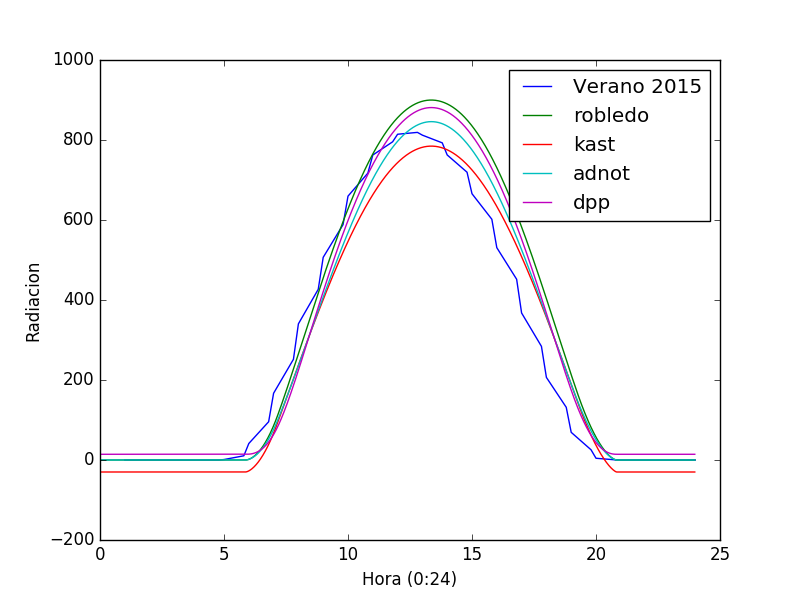
\includegraphics[width=12cm]{figures/verano2015.png}
		\caption{Modelo verano 2015}
	\end{center}
    \label{modelo_verano}
\end{figure}

La \textbf{radiación solar} varía debido a diversos factores de las variaciones locales en la atmósfera como el \textbf{vapor de agua}, las \textbf{nubes} y la \textbf{contaminación}; también a otros como la \textbf{latitud} y \textbf{longitud}, el \textbf{día del año} y la \textbf{hora del día}.

Por ejemplo, la \textbf{latitud} y \textbf{longitud} influyen en el grado de incisión de los rayos solares en la superficie y la radiación disminuirá cuanta más cantidad de nubes haya y más alta sea la \textbf{humedad}. Al contrario pasará con la \textbf{temperatura}, cuanto más altas sean las temperaturas indicará una mayor radiación. Otro factor que influye a la hora de medir la radiación, es el tipo de \textbf{superficie} donde se mida, ya que la reflexión de los rayos varía según el tipo. Como ejemplo, la nieve refleja un 85 por ciento de la radiación, al contrario del asfalto que solo un 2 por ciento.

Para llevar a cabo esta predicción en este proyecto se han utilizado como variables atmosféricas la humedad, la temperatura y la propia radiación solar. La manera de resolver este problema han sido algoritmos de ``Machine Learning'' (explicados en el capítulo \ref{makereference4}).

\section{Motivación}
\label{makereference1.1}

Hoy en día es cada vez más importante el uso de \textbf{las energías renovables} y así utilizar cada vez menos los combustibles fósiles. Esto es debido a que estas no producen gases de efecto invernadero que son los causantes del \textbf{cambio climático}, ni tampoco producen emisiones contaminantes, son inagotables y no generan residuos difíciles de tratar.

También tienen algunos inconvenientes como por ejemplo, el gran impacto visual que tienen y las grandes cantidades de terreno que se necesitan para poder conseguir una cantidad significante de energía. Además no siempre se obtiene la misma cantidad de energía. Depende, por ejemplo, de la cantidad de sol o de viento en ese momento.

Este último inconveniente es el que hace que las compañías productoras y distribuidoras sean reacias al uso de estas energías. Debido a la incertidumbre de \textbf{cuánta energía se va a producir}, es difícil desarrollar estrategias de compra de energía a otros productores y adecuación de su producción y capacidad de reserva.

En energías renovables como la eólica, los modelos predictivos disponibles actualmente son bastante precisos y su impulso es más fácil que otras como la energía solar la cual es más dificil de predecir.

Se podría decir que todavía no existen modelos \textbf{realmente buenos} para predecir la energía solar. Hay algunas empresas como \href{https://aleasoft.com/es/}{Aleasoft}, que realizan estudios predictivos obteniendo previsiones horarias en tiempo real desde un día hasta diez días, pero sería necesario conocer la producción con un intervalo \textbf{de una o dos horas.}

\section{Breve descripción del sistema}
\label{makereference1.2}

Este sistema cuenta con cuatro grandes módulos de trabajo para llevar a cabo su función: nodo, servidor de datos, servidor de resultados y visualizador de datos.

\subsection{Nodo}
\label{makereference1.2.1}
Encargado de recoger los datos necesarios, está formado por distintos sensores que recogen la información meteorológica necesaria y una pequeña placa programable encargada de enviar esta información al \textbf{servidor de datos}.

\subsection{Servidor de datos}
\label{makereference1.2.2}
El \textbf{servidor de datos}, es el encargado de recibir, almacenar y distribuir la información obtenida por el \textbf{nodo}.

\subsection{Servidor de predicción}
\label{makereference1.2.3}
Tiene como función recoger la información almacenada del servidor de datos, procesarla para obtener la predicción y enviarla al \textbf{visualizador de datos}. Puede estar, o no, en la misma máquina que el servidor de datos.

\subsection{Sistema de visualización}
\label{makereference1.2.4}
Muestra los resultados en forma de gráficas para facilitar su análisis.

\begin{figure}[htb]
    \begin{center}
        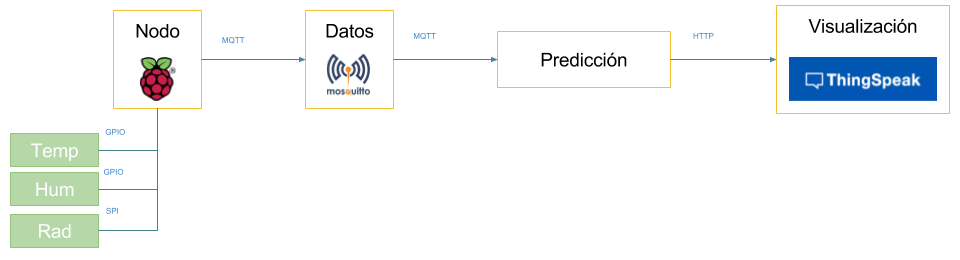
\includegraphics[width=15cm]{figures/diagrama-sistema.png}
        \caption{Diagrama de los componentes del sistema con sus protocolos de comunicación.}
    \end{center}
    \label{diagrama-sistema}
\end{figure}
